\chapter{Il Volante}

% Tutte le scelte che sono state prese hanno portato a raccogliere molte idee sul come doveva essere ridisegnata l'applicazione e grazie alla divisione del gruppo ha permeso di ...

Il confronto con gli altri membri del team ha permesso raccogliere molte idee che hanno dato frutto
a scelte tecniche che si sono rivelate nel concreto un buon punto di partenza per ridisegnare la nostra 
UI e costruire un dispositivo utile in tutte le sue possibili applicazioni.
Di conseguenza, per quanto riguarda la parte prettamente grafica e di funzionalità possibili, il confronto
è stato essenziale, l'influsso di idee da parte dei parecipanti ha fatto si che si delineassero dei requisiti
essenziali che non erano stati pesanti per la versione di Chimera.
Grazie a questo sono poi emersi i limiti dell'utilizzo del Volante mostrandoci cosa poteva essere sviluppato esternamente
per completare il quadro del progetto Telemetria, delineando l'assetto del team e gli obbiettivi per la stagione 2018/2019.

\section{Design della Applicazione}

% \textbf{ARGOMENTI}
% \begin{itemize}
%     \item come era il progetto e come è diventato (classe canbus, sistemazione switch che gestisce i messaggi, tabview e racing page)
%     \item funzionamento fsm (come funziona più o meno )
%     \item qt nel nostro caso come è stato utilizzato (class diagram e cross compilazione)
%     \item nuovi messaggi e nuove funzionalità integrate (calibrazione pedaliera, utilizzo dei manettini per le pompe e per il traction control)
% \end{itemize}

\begin{figure}[hbt!]
    \centering
    \includegraphics[width=0.75\textwidth]{./figures/cd.pdf}
    \caption{Class Diagram di Novembre 2018}
\end{figure}

Il progetto è composto da un file \emph{.pro} che ha come utilità quella di raggrupare tutte le componenti
del progetto, dai file compilabili \emph{.cpp} e \emph{.h} al \emph{qml.qrc}, che ci permette di raccogliere 
tutti gli assets principali, quindi immagini e i file \emph{.qml}.
Questo permette di mantere una struttura ordinata nella cartella del progetto e grazie al comando \emph{qmake},
che permette di generare il makefile specifico per la piattaforma in cui si sta facendo la build, permette di automatizzare 
tante procedure senza dover passare dal loro IDE proprietario. 
Durante lo sviluppo si è reso necessario documentare tutto il codice, perchè fino a quel momento non presentava commenti 
o guide in grado di spiegare le scelte prese e come funzionano alcune decodifiche dei messaggi, sia per il FE che per il BE. 
La repository inoltre mostrava difficolta nell'essere mantenuta quindi si è deciso di riorganizzare in sottocartelle e 
rimuovere le parti di codice non più utili in fase di test, soprattutto per la parte di qml in cui erano presenti pagine di prova e componenti
non più utilizzati.  

Il programa è diviso in tre parti:

\begin{itemize}
    \item La lettura dei dati dal Can-Bus (Canbus) 
    \item Lo stato della macchina (CarStatus)
    \item Il Front-End
\end{itemize}

% CanBus
La classe \emph{Canbus} si occupa di gestire l'invio e la ricezione dei messaggi via Can-Bus (SocketCan).
L'evoluzione, rispetto all'anno precedendete, è presente a lato hardaware, fornendo alla scheda la possibilità
di poter comunicare in Can-Bus direttamente, senza dover passare 
per una seriale e un dispositivo esterno visto come "gateway".
A livello software questo ha permesso di poter utilizzare la libreria 
di Qt basata sui driver Linux di cui ho già parlato.
Questa classe si occupa quindi di inviare messaggi quando richiesto dall'utente o in automatico, 
di ricevere e settare i valori nella classe \emph{CarStatus}.
% CarStatus
\emph{CarStatus} si occupa di salvare i valori letti precedentemente dal Can-Bus, 
in strutture dati in grado di essere lette dall'UI 
e se ritenuto necessario aggiornare l'interfaccia. 
Questo non era sempre presente nella versione precedente perchè essendo 
un prodotto in via di sviluppo non sempre questa scelta ci è sembrata la più veloce
dovendo aggiornare il codice in tempi brevi.
% QPROPERTY nel dettaglio
Il vanataggio di Qt è evidente quando si usano le sue librerie, 
in particolare se consideriamo l'aggiornamento di una digital dash la prima cosa che 
cambia notevolmente il workflow sono le sue \textbf{property}
che permetteno ai "meta-object" di poter comunciare tra di loro attravers il sistema \emph{signal} and \emph{slot}.
Le property si basano su funzioni per segnalare il cambiamento di un valore (NOTIFY), 
la sua lettura (READ), la sua scrittura (WRITE) e altre non utilizzate nel nostro caso. 
Questo permette di rendere accessibile un dato o una struttura dati dal Frontend al Backend 
e viceversa, in caso di input da parte dell'utente.
Il meccanismo inizialmente può sembrare macchinoso, poi, essendo mnemonico, può essere riutilizzato in molte 
situazione e, in termini di performance, permette di velocizzare l'accesso ai dati. 
Come introdotto precedentemente, senza conoscere il framework può sembrare più intuitivo utilizzare delle funzioni
in lettura e in scrittura pensate ad hoc, ma questa oltre a non essere la prassi influisce
sulle performance e in progetti grandi non permette di mantenere un'architettura precisa.
In termini di performance non sono stati fatti test mirati alla raccolta di dati sulla velocità di lettura e scrittura, 
ma abbiamo visto che alcuni valori non venivano letti soprattutto 
quando l'eseguibile è sotto stress per i continui messaggi Can-Bus.

\subsection{Interfaccia 2017}

% interfaccia con tab view d una pagina utilizzata in fase di run con info generiche, le altre con info specifiche
% si vedrà nel prossimo capitolo un approfondimento e come questa scelta sia stata riconsiderata

\begin{figure}[h!]
    \centering
    \begin{minipage}{0.5\textwidth}
        \centering
        \includegraphics[width=0.8\textwidth]{./figures/oldUI/tabErrors.png}
        \caption{Interfaccia di Chimera - Tab View}
    \end{minipage}\hfill
    \begin{minipage}{0.5\textwidth}
        \centering
        \includegraphics[width=0.8\textwidth]{./figures/oldUI/racingPage.png}
        \caption{Interfaccia di Chimera - Racing Page}
    \end{minipage}
\end{figure}

La digital dash di Chimera era stata pensata più in un ottica di test,
dividendo in due parti le funzionalità.
La prima parte, di configurazione e di lettura dello stato della sensoristica 
in una Tab View.
La Tab View necessitava principalmente di due tasti, uno per muoversi ed uscire dalla 
Tab e un altro per poter entrare e inviare il comando. Considerando il caso della \emph{Tab Errors} 
con il tasto in alto a sinistra è possibile spotarsi su quella vista, entrare con il tasto in basso a destra
e mandare il comando con lo stesso, per poi uscire con il tasto in alto a destra. 
La seconda parte, la \emph{Racing Page}, dove si poteva vedere lo stato di carica dei pacchi batteria,
i Kw erogati, lo stato della macchina e comunicare via radio con il muretto, funzione che non è mai stata implementata seriamente.
Nei prossimi capitoli verrà analizzata in modo più completo l'interfaccia e la \emph{Racing Page}, 
prendendo in considerazione le scelte fatte per Chimera Evoluzione.

\subsection{Finite State Machine}

\begin{figure}[hbt!]
    \begin{center}
        \begin{tikzpicture}[scale=0.2]
            \tikzstyle{every node}+=[inner sep=0pt]
            \draw [black] (40.5,-40.7) circle (3);
            \draw (40.5,-40.7) node {$Run$};
            \draw [black] (12.3,-22.1) circle (3);
            \draw (12.3,-22.1) node {$Idle$};
            \draw [black] (12.3,-22.1) circle (2.4);
            \draw [black] (67.9,-22.1) circle (3);
            \draw (67.9,-22.1) node {$Setup$};
            \draw [black] (15.3,-22.1) -- (64.9,-22.1);
            \fill [black] (64.9,-22.1) -- (64.1,-21.6) -- (64.1,-22.6);
            \draw [black] (65.42,-23.78) -- (42.98,-39.02);
            \fill [black] (42.98,-39.02) -- (43.92,-38.98) -- (43.36,-38.15);
            \draw [black] (42.98,-39.02) -- (65.42,-23.78);
            \fill [black] (65.42,-23.78) -- (64.48,-23.82) -- (65.04,-24.65);
            \draw [black] (64.9,-22.1) -- (15.3,-22.1);
            \fill [black] (15.3,-22.1) -- (16.1,-22.6) -- (16.1,-21.6);
            \draw [black] (38,-39.05) -- (14.8,-23.75);
            \fill [black] (14.8,-23.75) -- (15.2,-24.61) -- (15.75,-23.77);
        \end{tikzpicture}
    \end{center}
    \caption{Finite State Machine del Volante}
\end{figure}

Il funzionamento della macchina a stati del Volante è gestita dall'ECU. 
La FSM rispecchia il lavoro del Team del Controllo, lo scopo del Volante è quello di permettere al pilota 
di poter cambiare, in sicurezza, lo stato. In sicurezza perchè la maggior parte dei controlli avvengono lato ECU
e il Volante è stato sviluppato per rendere il più intuitivo e a prova di errori umani la procedura di accensione. 
Tramite l'interfaccia possiamo inviare richieste e se sono accettate dall'ECU, quindi se è possibile cambiare stato dallo stato di partenza,
effettua i controlli e le richieste a chi di dovere e risponde in modo positivo.
La monoposto, successivamente all'accensione del pacco low voltage (BMS LV) si troverà in \textbf{IDLE}, 
da qui se non si presentano errori si può mandare una richiesta di \textbf{START} 
e se la risposta è positiva possiamo quindi passare alla fase di \textbf{SETUP}. 
Durante questa richiesta l'ECU si occuperà di chiedere al pacco high voltage (BMS HW) di accendersi chiudendo in serie il primo e il secondo AIR. 
Se l'accensione termina con successo il BMS HV risponde all'ECU, la quale poi conferma al Volante lo stato Setup.
Il pilota ora ha due possibilità: richiedere l'accensione degli Inverter, e se questa procedura termina correttamente
sarà possibile mandare una richiesta per entrare nella fase di \textbf{RUN}, in cui l'ECU abilita l'utilizzo della pedaliera.
Oppure mandare una richiesta di spegnimento del pacco batteria high voltage attraverso il comando di \textbf{STOP}.
Il Volante ha due possibilità quando si trova in RUN: 

\begin{itemize}
    \item Errori: In base al tipo di errore che riscontra l'ECU può fare richiesta di spegnimento al pacco low voltage o passare in fase di IDLE.
    \item SetUp: Richiesto dal pilota, disabilita la pedaliera e bisogna ripetere la procedura di accensione degli inverter. 
\end{itemize} 

Bisogna sempre tenere in considerazione che le variabili di stato che vengono modificate dipendono
dai messaggi presenti nella rete e che hanno come destinario il Volante, dovendo sempre ricevere un feedback da parte dall'ECU
L'utente, che sia il pilota o chi sta testando la macchina, ha poche responsabilità in caso di errore.
Gli errori che si possono riscontrare sono da verificarsi nei cambiamenti di stato o negli stati stessi della FSM e dalle componenti
della monoposto per possibili malfunzionamenti.  
Solo i manettini, per come è stato scritto il codice, permettono di aggiornare l'interfaccia senza ricevere un feedback
in quanto il messaggio sullo stato di connessione del Volante è inviato in ogni 500ms, si per mostrare la presenza nella rete
che per condividere le preferenze del pilota.


\newpage


\subsection{Cross Compilazazione}


\begin{figure}[hbt!]
    \centering
    \includegraphics[width=0.75\textwidth]{./figures/cross-compilazione.png}
    \caption{Guida Cross Compilazione del Team \cite{cross-compilazione}}
\end{figure}


% APPROCCIO ALLO SVILUPPO SUL SISTEMA EMBEDDED

L'approcio allo sviluppo del progetto si è diviso in due parti.
La prima parte è stata buildare il progetto sul laptop ed eseguirlo, 
cambiando la classe bottoni per poter avere gli input da tastiera e utilizzare 
una interfaccia virtuale per la comunicazione Can-Bus.
Per l'utilizzo dei bottoni si è deciso di mantenere la posizione de tasti del Volante portandoli sulla tastiera.
I quattro tasti funzione sono disposti a "quadrato" sono diventati "Q-A-D-R", 
per il manettino delle mappe invece sono stati utilizzati i numeri fino al 6.
Per quanto riguarda invece gli altri due manettini i test sono stati fatti via \emph{ssh} valutando l'input 
e il loro cambiamento di stato, successivamente sono stati portati anche loro su tastiera usando in ordine 
le lettere della parte destra della tastiera quindi per le pompe "T-Y-U-I-O-P" e per il controllo "F-G-H-J-K-L".    
La seconda parte ci ha messo più in difficoltà perchè inizialmente abbiamo avuto problemi di compatibilità 
con il sistema operativo del target device e la sua versione di Qt che non risultava congruente con la nostra.
Precedentemente il Volante era stato compilato con la versione 5.7 di Qt, con il nuovo sistema operativo, buildato
con Buildroot, potevamo installare solamente la 5.10.1. 
Questo inizialmente è apparso come un problema da poco ma quando abbiamo visto che per una classe, \emph{QCanBus}, 
le funzioni non erano più presenti nello stesso modo abbiamo dovuto rivedere la procedura di cross-compilazione per
riuscire a compilare il codice con la versione successiva di Qt. 
Allineate queste divergenze, gli approcci che abbiamo considerato cercando nella documentazione di Qt e nei forum
sono due:

\begin{itemize}
    \item Deploy su Target Board
    \item Deploy in Locale 
\end{itemize}

Noi abbiamo deciso di compilare il progetto dal nostro host e poi spostare l'eseguibile sul target device, automatizzando la procedura attraverso 
uno script in bash utilizzando l'auto-login di \emph{ssh}, il kill del processo in esecuzione per poi poter trasferire la versione appena compilata ed eseguirla.
La scelta è motivata dal poter lasciare il target device più leggero e non avere necessità di esso nella fase di compilazione, ma solo per eseguirlo.
Per compilare il codice del Volante da un dispositivo linux abbiamo dovuto cross-compilare, 
questo significa che mediante un compilatore esterno abbiamo "emulato" il sistema target compilando il sorgente 
come se fossimo l'host di riferimento. Così da poter eseguire il file su un architettura diversa da quella del host di origine.
Questa è stata la difficoltà più grande riscontrata con l'utilizzo di Qt per dispositivi ARM, abbiamo dovuto trovare il modo di testare 
in locale l'applicazione, senza avere a disposizione il dispositivo. 
La procedura per avere l'ambiente adatto a cross-compilare, considerata la versione open-source e
non fornendo la tool-chain proprietaria, è molto lenta e richiede ore per poterla portare a termine.
La guida che abbiamo ottenuto prevede il montare il sistema operativo del target device (in questo caso non lo stesso, ma raspbian lite) 
e installare le librerie di Qt, per poi avere il qmake necessario a generare il makefile adatto allo scopo.

% Conclusioni sulla cross-compilazione

La nostra inesperienza nel settore ci ha fatto impiegare molto tempo nella risoluzione 
di problemi anche banali, ma ci ha anche permesso di imparare tanto e soprattutto di capire
che esistono soluzioni più semplici, ancora da testare, delle quali parlerò meglio nelle valutazioni.

\section{Redesign della Applicazione}

% problemi dell'interfaccia a livello software e come sono stati risolti 
% disegno su carta con low fidelity prototype --> mockup

L'utilizzo del Framework Qt ha portato numerosi vantaggi quando è stato deciso di ridisegnare l'interfaccia.
Inizialmente gli oggetti che componenvano la UI erano tutti nel meta linguaggio \emph{QML} utilizzato da Qt, questi oggetti si basano 
sul linguaggio JavaScript e permettono di attribuire proprietà all'interfaccia per poi essere gestita dagli eventi generati dal codice C++.
Questo in partenza è risultato essere un limite quando si è deciso di utilizzare il formato \emph{.png} per comporre la strumentazione, 
ma successivamente abbiamo riscontrato la predisposizione di Qt all'utilizzo di immagini.

\subsection{Dal Low Fidelity Prototype al primo Mockup}

Tutto è iniziato da un foglio di carta, un A3 per la precisione, dopo aver raccolto tutti requisti da parte del team
abbiamo iniziato a disegnare e a pensare come poteva essere aggiornato il Volante per venire incontro alle nostre necessità.

Le persone coinvolte nel redesign dell'applicazione sono state:

\begin{itemize}
    \item Davide Farina: Pilota e quindi primo utilizzatore del Volante
    \item Luca Martinelli: Sviluppatore e utilizzatore del Volante come debugger per la macchina
    \item Laura Scoccianti Designer, che si è occupata di portare l'interfaccia da Low Fidelity Prototype a Mockup 
\end{itemize}


\begin{figure}[hbt!]
    \centering
    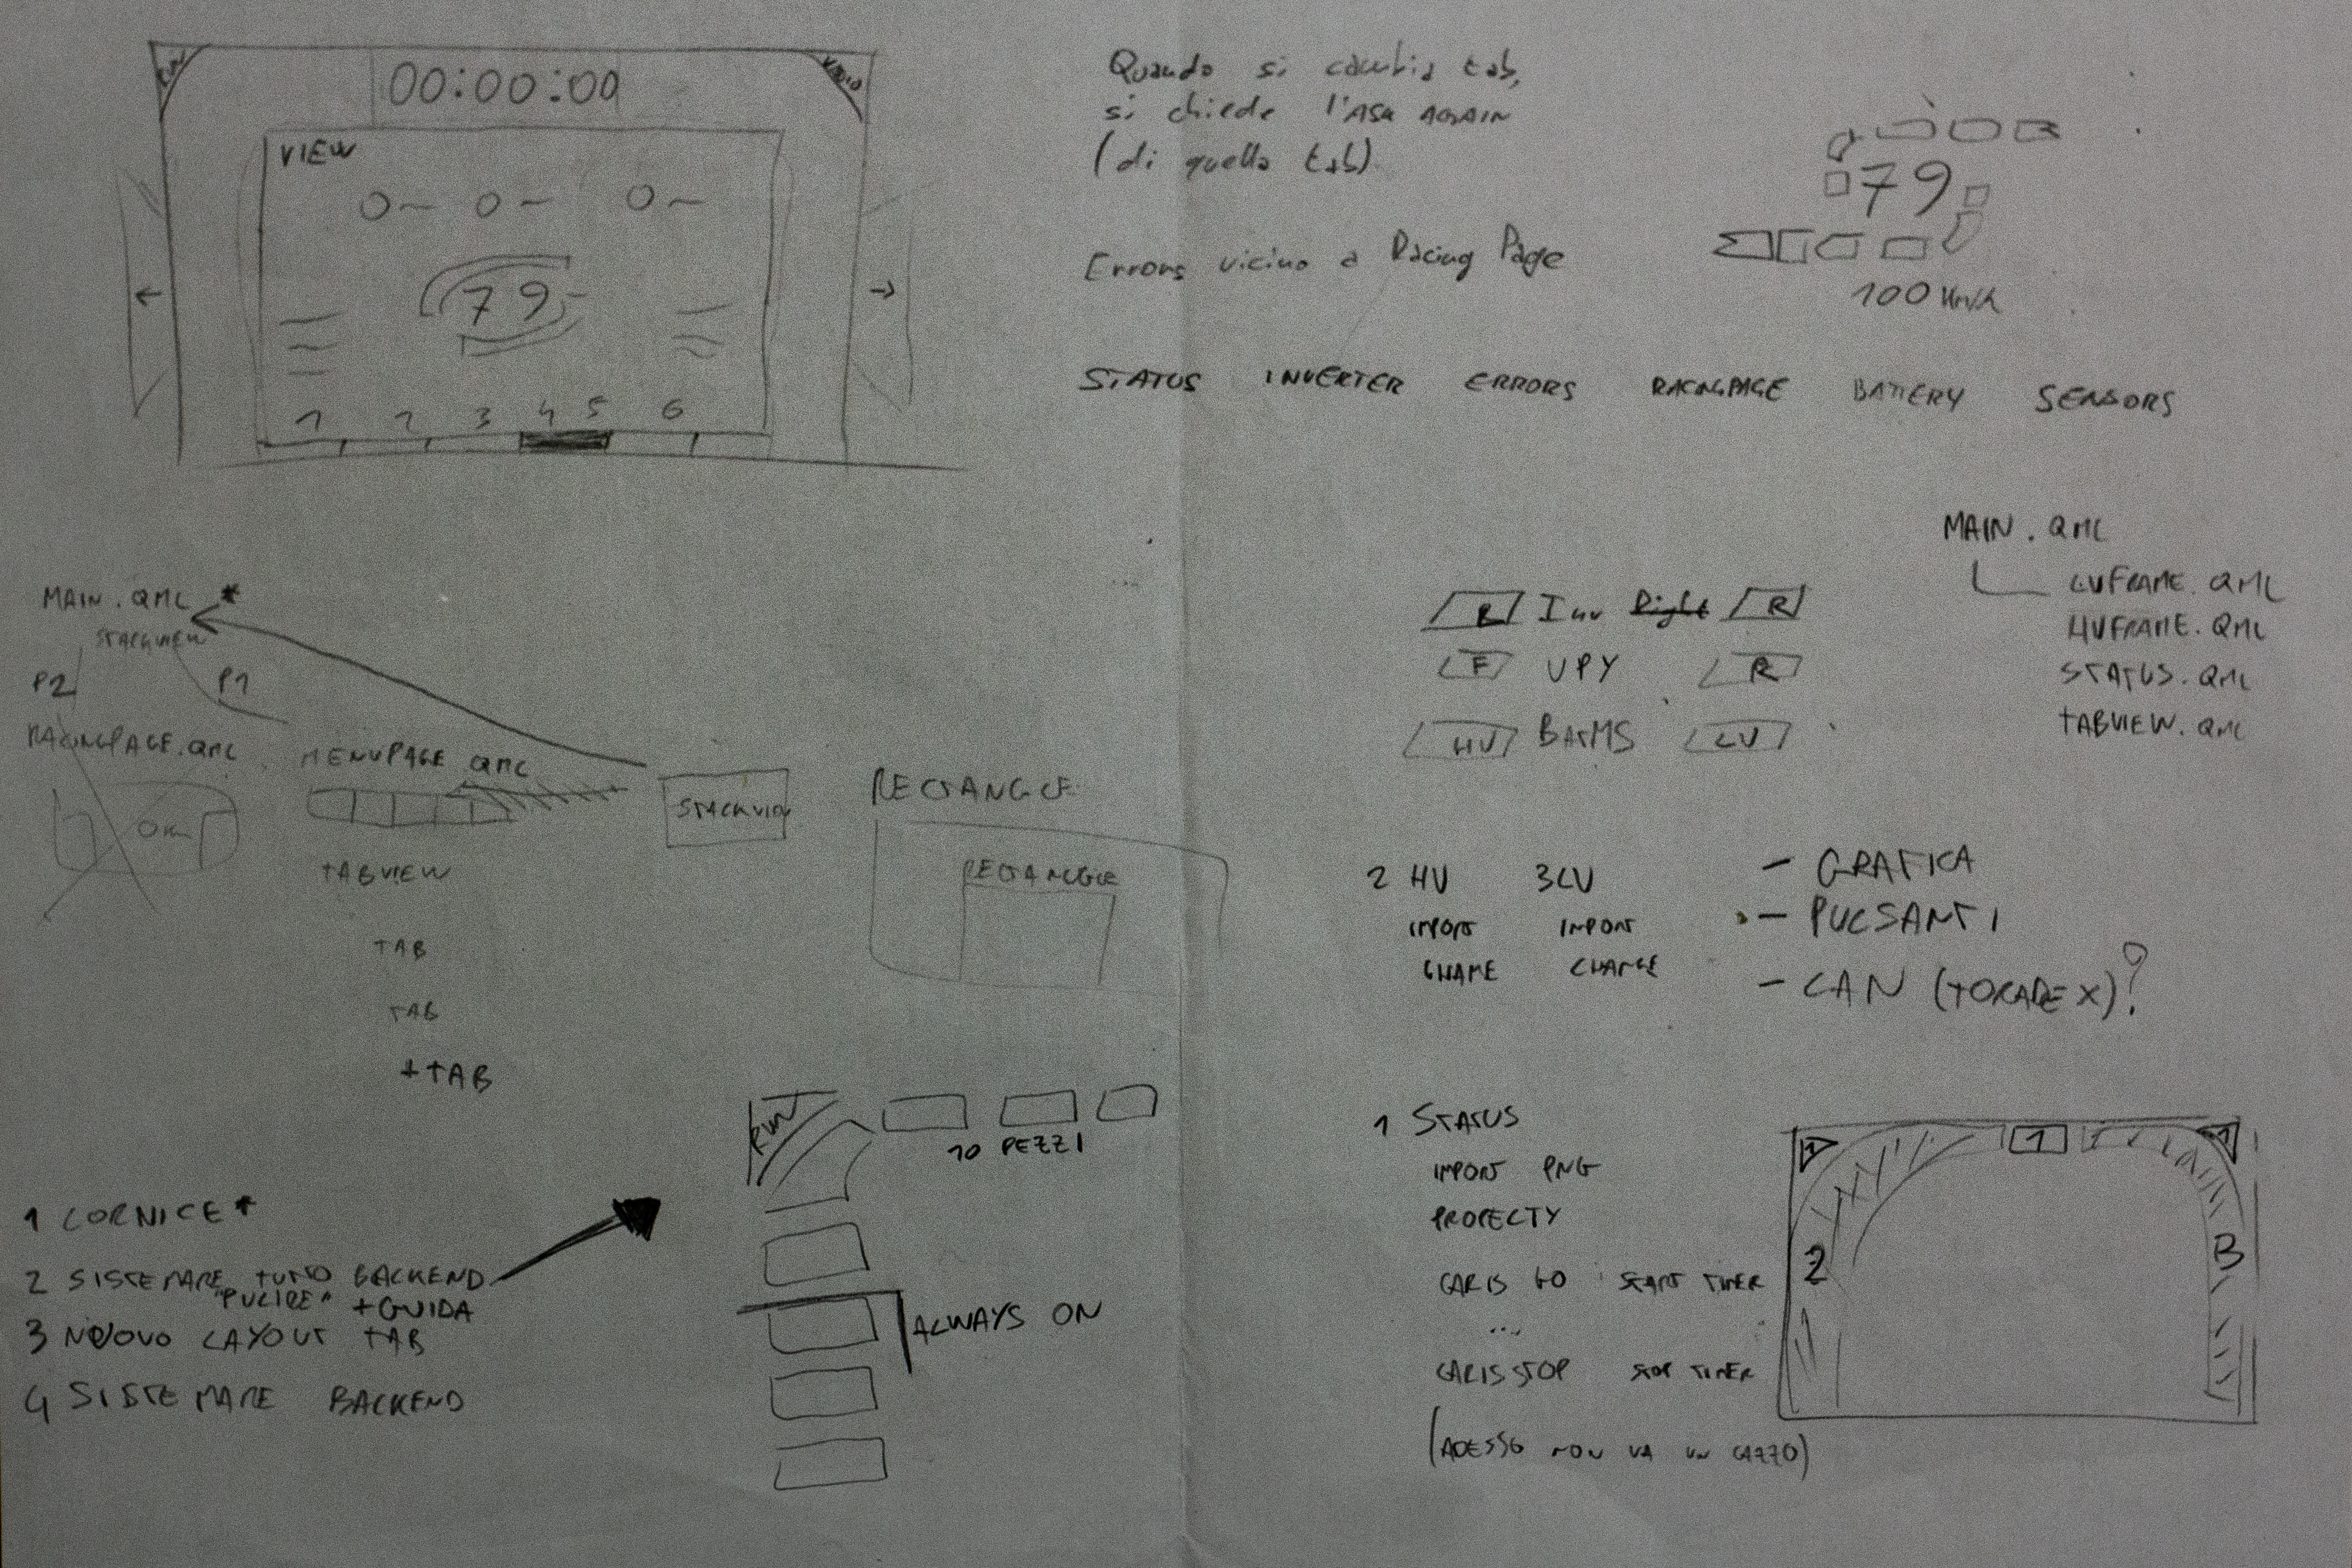
\includegraphics[width=0.75\textwidth]{./figures/lowfidelityprototype.jpg}
    \caption{Low Fidelity Prototype}
\end{figure}

% disegno

% cosa abbiamo deciso quindi? cornice hv e lv sempre presenti, ridimensionamento oggetti non necessari

Il Low Fidelity Prototype ha preso subito forma, ed una delle cose che è stata in primo luogo fatta presente è
la possibilità di potersi muovere in modo intuitivo nelle Tab, quindi senza dover passare da una vista Tab View a una pagina singola
come era in precedenza.
La giustificazione nasce dall'esigenza di una migliorare usabilità, in quanto anche in fase di \emph{RUN} deve essere possibile cambiare Tab.
Questo ha fatto si che la \emph{Racing Page} dovesse essere integrata nella vista a Tab oppure di cambiare completamente layout.
Una delle prime proposte è stata la visuale dello stato della macchina in tutte le pagine, insieme al livello di carica dei due pacchi 
batteria. Questo ci ha messo davanti ad una scelta, integrare questi indicatori all'interno di ogni pagina o utilizzarli come cornice. 
La seconda scelta si è rivelata la più efficace e semplice da implementare, senza dover badare alla riscrittura di codice in più parti.
Un'altra funzionalità, che a livello estetico ha permesso di "animare" l'interfaccia
in fase di test con il tractive system disattivato, è stata l'inserimento di due slider per i sensori della pedaliera.
L'accelleratore e il freno nella Racing Page del Volante sono stati pensati per poter dare un feedback sulla pressione completa, quindi quando 
si è al 100\% durante l'accellerazione.  
Una proposta che è stata poi scartata è stata la possibilità di visualizzare in una Tab dedicata la dinamica del veicolo potendo
valutare la \emph{g-force} letta dalle IMU, l'implementazione si basava su un grafico a radar stile Formula 1.

Per quanto riguarda la scelta di stile e colori da utilizzare per l'interfaccia ci siamo ispirati al mondo della Formula E
e dei videogiochi Racing, utilizzando colori molto accesi e facili da distinguere anche in situazioni di scarsa luminosità.
Questo è uno dei punti forte della nostra interfaccia, la cura dei particolari e soprattutto la scelta dei colori è 
stata molto discussa dovendo mostrare e far percepire al pilota in breve tempo il cambiamento di certe condizioni.  

Ognuna delle persone coinvolte ha dato la sua opinione sulla fattibilità delle funzioni da integrare e sulla loro utilità
votando su quali erano da mantenere e altre da scartare o mettere come ultime nel processo di integrazione.
Così facendo si è definito il Gantt per l'integrazione delle funzionalità. 

Successivamente è stato necessario portare questo prototipo in qualcosa di più definitivo e integrabile nell'interfaccia.
Il risultato è stato reso possibile da Laura Scoccianti, che si è da sempre occupata della parte grafica del team, in questo caso 
ha portato il nostro Low Fidelity Prototype in un High Fidelity Prototype utilizzando un software per la grafica.
Elaborato il primo mockup, dopo averne discusso con i membri del Team siamo passati all'integrazione, ogni singola parte della UI
è stata poi esportata in formato \emph{.png} e integrato con le funzioni già presenti e in corso di sviluppo della macchina. 

Questo tipo di approccio è stato reso possibile dalla definizione già in partenza della composizione del team e delle task
e basando il processo di sviluppo sui clienti interni ed esterni visti come il "pilota", il "tester" e chi si è occupato della realizzazione.

\subsection{Integrazione della nuova UI del Volante}

% probelma della cornice - risolta rendendo la tab view più piccola ed eliminando i nomi delle tab, mostrando solo come indicatore su quale tab si è
% integrazione dell'accelleratore freno nella racing page
% utilizzo dei paddle per potersi muovere più agevolemente nell'interfaccia e aumentare le funzionalità dei quattro tasti sulla maschera frontale
% aprendo al'integrazione di funzioni come pressione di più tasti insieme

\begin{figure}[hbt!]
    \centering
    \includegraphics[width=0.75\textwidth]{./figures/primoMockUpUI.jpg}
    \caption{Primo Mockup}
\end{figure}

% integrazione della cornice
Il problema della cornice da integrare è stato risolto ridimensionando la Tab View per fare spazio 
agli indicatori del pacco HV,LV e inserendo il timer non ancora implementato su Chimera. 
L'integrazione ha dato problemi nello sviluppo perchè la UI non era mai stata pensata per essere reponsive, in quanto in un ambito come questo non 
è effettivamente richiesto. 
Le difficoltà sono apparse nel dover integrare le funzioni per gestire il valori da visualizzare inserendoli allo stesso livello nel \emph{main.qml}
Tab e corince.
% orientamento posizione tab
Il ridimensionamento delle Tab ha portato alla perdita della visualizzazione del nome della Tab in cui si è, fattore molto importante
perchè la mancanza di riferimenti durante l'utilizzo del programma peggiora l'esperienza d'uso.
La soluzione è stata indicare la posizione delle Tab nella parte inferiore del display e, grazie l'utilizzo dei paddle, sapere se bisogna andare a destra o a 
sinistra per visualizzare la Tab desiderata. 
In più prima non era possibile tornare indietro nelle Tab ma si potevano percorrere solo da sinistra verso destra.
Questo fa parte dei compromessi che non si sono rivelati negativi, anzi l'interfaccia di Chimera Evoluzione nasce dalle mancanze riscontrate da Chimera.
Una nota sull'interfaccia risulta doverosa, questo non è un dispositivo adatto e utilizzato da tutti, ma solo da chi è stato istruito 
sul funzionamento della macchina e sulla sua parte elettronica. I nostri piloti sono all'interno del team e lavorano con noi
allo sviluppo della monoposto.

\begin{figure}[h!]
    \centering
    \begin{minipage}{0.5\textwidth}
        \centering
        \includegraphics[width=8cm]{./figures/imageracing.jpg} % first figure itself
    \end{minipage}\hfill
    \begin{minipage}{0.5\textwidth}
        \centering
        \includegraphics[width=8cm]{./figures/imagetutorial.jpg} % second figure itself
    \end{minipage}
\end{figure}

% pedaliera
L'integrazione dei sensori della pedaliera nella \emph{Racing Page} invece non ha riscontrato particolari problemi, è stata rideimensionata la
grandezza del rettangolo in cui dovevano essere collocati i \emph{.png} che hanno mantenenuto le dimesnioni del display (il layer in questo caso)
quando sono state esportate è stato solo macchinoso farli risultare nella posizione corretta durante l'aggiornamento dei KW.
Questo ha anche permesso di rivalutare la grandezza dei font e, verificando direttamente con il pilota, la nostra grafica ci ha fornito i file con le dimensioni
aggiornate che si è trattato solo di ri-integrare nella interfaccia.
% velocità
Un'altra integrazione, dovuta all'aggiunta degli encoder sulle ruote, è stato il calcolo della velocità, oltre al valore dei KW richiesti ora
è possibile visualizzare in \emph{Racing Page} anche la velocità calcolata dalle schede che si occupano della sensoristica.
% radio-feedback
Il sistema di comunicazione radio, che è stato lentamente abbandonato nel corso dello sviluppo della monoposto, ha lasciato spazio, utilizzando
il suo tasto in alto a destra nell'interfaccia, all'invio di un marker in CAN che permette al pilota di segnalare in un certo momento che è successo 
qualcosa.
% calibrazione pedaliera
Durante lo sviluppo si è reso necessario integrare una procedura per calibrare la pedaliera, questo ha messo in risalto alcune criticità 
nel come era stata pensata la UI mostrando possibili approcci diversi.
La calibrazione è stata implementata potendo muoversi nei vari sensori con una procedura interattiva segnalando all'utente se ha effettivamente
concluso una delle fasi. Le criricità sono apparse nel momento in cui bisognava mostrare il feedback, cambiando solamente il testo a volte non si permette all'utente 
di accorgersi se ha effettivamente concluso quella parte. Il problema è stato preso e analizzato e le soluzioni saranno visibili nella prossima implementazione
del Volante per la stagione 2019/2020.  







\newpage






\section{Funzionalità delle diverse pagine}

% spiegazione struttura grafica della pagina, per poi finire nella racing page

L'interfaccia del Volante di Chimera Evoluzione è composta da più Tab disposte in serie che permettono di seguire in ordine
la procedura di accensione e di test standard della monoposto. Alcune funzionalità sono state inserite solo a livello grafico
e per dare forma all'interfaccia, sono state successivamente implementate su Chimera Evoluzione. 
I nomi delle Tab hanno subito modifiche perchè per come era stata concepita non erano presenti 
vere relazioni tra il nome, le funzionalità e ciò che doveva essere visualizzato. 
La versione mostrata è quella standard utilizzata per i test. 

\subsection{Warning Tab}

\begin{figure}[h!]
    \centering
    \begin{minipage}{0.5\textwidth}
        \centering
        \includegraphics[width=0.9\textwidth]{./figures/UI/tabWanings.png}
        \caption{Chimera Evoluzione - Tab Warnings}    
    \end{minipage}\hfill
    \begin{minipage}{0.5\textwidth}
        \centering
        \includegraphics[width=0.9\textwidth]{./figures/oldUI/tabErrors.png}
        \caption{Chimera - Tab Errors}
    \end{minipage}
\end{figure}

La prima Tab, chiamata anche \emph{Warning Tab}, mostra lo stato della sensoristica.
Diversamente dalla \emph{Errors Tab}, i warnings non sono errori critci e servono 
solo a informare il pilota se certi sensori non funzioneranno come dovrebbero.
Inizialmente erano presenti alcuni sensori che sono stati rimossi perchè non più necessari,
e la richiesta di update è stata resa automatica per poter aumentare lo spazio nella Tab.  
Nelle prime fasi di test questa funzionalità si è rivelata molto utile perchè ci ha permesso
di vedere sin dalla prima accensione se i dispositivi erano collegati e funzionavano.
Con la presenza di warnings è possibile abilitare il tractive system e utilizzare la macchina, 
se dovessero apparire degli warnings durante la fase di \emph{Run} questo non non cambierebbe lo stato,
cosa che invece accade per gli errori.

\subsection{Error Tab}

\begin{figure}[h!]
    \centering
    \begin{minipage}{0.5\textwidth}
        \centering
        \includegraphics[width=0.9\textwidth]{./figures/UI/tabErrors.png}
        \caption{Chimera Evoluzione - Tab Errors}    
    \end{minipage}\hfill
    \begin{minipage}{0.5\textwidth}
        \centering
        \includegraphics[width=0.9\textwidth]{./figures/oldUI/tabStatus.png}
        \caption{Chimera - Tab Status}
    \end{minipage}
\end{figure}

La seconda Tab, chiamata anche \emph{Errors Tab}, permette di visualizzare la panoramica degli errori presenti in macchina, 
se sono presenti errori critci andranno verificati con gli interessati e risolti per poter entrare nella fase di \emph{Setup}.
In questa Tab è stata ripensata la procedura di accensione, cambiando il comando di \emph{Ask Again} con il comando di \emph{Stop}
ed è stata ridimensionata per poter inserire altre scheda come ad esempio la pedaliera.
Se non sono presenti errori, possiamo mandare il messaggio di \emph{Start} e successivamente poter tornare nella fase \emph{Idle}
tramite il comanodo \emph{Stop}.


\newpage


\subsection{Status Tab}

\begin{figure}[h!]
    \centering
    \begin{minipage}{0.5\textwidth}
        \centering
        \includegraphics[width=0.9\textwidth]{./figures/UI/tabStatus.png}
        \caption{Chimera Evoluzione - Tab Status}    
    \end{minipage}\hfill
    \begin{minipage}{0.5\textwidth}
        \centering
        \includegraphics[width=0.9\textwidth]{./figures/oldUI/tabInverter.png}
        \caption{Chimera - Tab Inverter}
    \end{minipage}
\end{figure}

La terza Tab, chiamata anche \emph{Tab Status}, mostra lo stato della precharge e degli inverter.
Da qui, grazie ai led, possiamo vedere se non comunicano, quindi led grigio, se sono abilitati o no (rosso e verde).
Questa Tab permette di accendere o spegnere gli inverter facendone richiesta.
Questa procedura deve essere effettuata prima di entrare nella \emph{Racing Page} per poter entrare nella modalità \emph{Ready To Drive}.
Non è possibile entrare in questa modalità, se non vengono abilitati, in quanto di default sono impostati ad off.

\subsection{Racing Page}

\begin{figure}[h!]
    \centering
    \begin{minipage}{0.5\textwidth}
        \centering
        \includegraphics[width=0.9\textwidth]{./figures/UI/racingPage.png}        
        \caption{Chimera Evoluzione - Racing Page}    
    \end{minipage}\hfill
    \begin{minipage}{0.5\textwidth}
        \centering
        \includegraphics[width=0.9\textwidth]{./figures/oldUI/racingPage.png}
        \caption{Chimera - Racing Page}
    \end{minipage}
\end{figure}

La quarta Tab, chiamata anche \emph{Racing Page} è la più importante e la più curata dal punto di vista del design.
Senza doversi spostare in altre Tab si è in grado di avere una visione generale della macchina.
Da qui si può interagire con la sezione in alto a sinistra che mostra lo stato della macchina (idle, setup, run, stop)
attraverso il comando di \emph{Run} e il relativo comando di \emph{Stop} che nel primo caso abilitano l'utilizzo della pedaliera
e nel secondo permettono di tornare nella fase di \emph{Setup}, disabilitando gli inverter.
Nella parte più alta sono presenti tre led che mostrano se il controllo è stato abilitato e in sequenza 
i possibili warning o errors presenti in macchina in caso di malfunzionamenti durante la fase di \emph{Run}.
L'introduzione di questi led è stato inoltre utile per evitare che il pilota possa entrare, se non abilitato, nella fase di \emph{Run}
tenendo sempre a mente che il Volante non si occupa di gestire i casi di errore, ma solo di visualizzarli.
Le funzioni disponibili, come già spiegato, sono definite dalla macchina a stati.
Al centro dello schermo è posizionato il valore, in KW, richiesto ai motori, 
attorno possiamo trovare in azzuro quanto viene premuta la pedaliera e in rosso lo stato del freno per dare un feedback al pilota 
mostrandogli, in accellerazione, quando si trova al 100\%.
Appena sotto invece è posizionata la velocità letta dagli encoder, fino ad arrivare alla mappa scelta.
In questa sezione il pilota può vedere in che mappa si trova, scelta grazie all'ausilio dei manettini.
Le mappe permettono di selezionare, in \%, la potenza da erogare ai motori, la prima mappa abilita la retromarcia (-20\%), 
dalla seconda in poi invece incrementa del 20\% fino ad arrivare alla mappa 6 che indica il massimo erogabile.  
Il selettore delle mappe oltre ad essere molto utile in fase di test, soprattutto per verificare in linea generale la sicurezza della macchina 
apre molte possibilità in termini di personalizzazione della guida. 
Il pilotta infatti oltre a questo manettino ne ha a dispozione altri due: uno per impostare il traction control e l'altro per il sistema di cooling. 
Grazie al primo il pilota può decidere se abilitare il torque vecoring, disattivarlo e utilizzare o no lo slip control e con l'ausilio del secondo
può impostare, manualmente, l'utilizzio delle pompe che indipendentemente da questo funzionano autonomamente.    
Rispettivamente sulla parte sinistra e destra troviamo lo stato del pacco lov voltage e high voltage con le loro temperature e voltaggio.
In più, durante la fase di test, si è reso necessario mostrare la temperatura degl inverter, da cui si è deciso di inserire questi dati 
congruentemente alla posizione degli inverter in macchina, quindi sinistra per l'inverter di sinistra e destra per l'inverter di destra.

\subsection{Battery Tab}

\begin{figure}[h!]
    \centering
    \begin{minipage}{0.5\textwidth}
        \centering
        \includegraphics[width=0.9\textwidth]{./figures/UI/tabBattery.png}
        \caption{Chimera Evoluzione - Tab Battery}    
    \end{minipage}\hfill
    \begin{minipage}{0.5\textwidth}
        \centering
        \includegraphics[width=0.9\textwidth]{./figures/oldUI/tabBattery.png}
        \caption{Chimera - Tab Battery}
    \end{minipage}
\end{figure}

La quinta Tab, chiamata anche \emph{Battery Tab}, permette di visualizzare lo stato di carica del pacco batterie High Volage e Low Voltage.
Per entrambe è presente la temperatura minima, massima e media della temperatura e della carica dei due pacchi.
Questa Tab è da utilizzare in fase di test, in quanto al pilota non avrà, o solo in pochi casi particolari, 
la necessità di sapere lo stato delle celle. Le informazioni più generali sono presenti invece nella \emph{Racing Page}.  


\subsection{Sensor Tab}

\begin{figure}[h!]
    \centering
    \begin{minipage}{0.5\textwidth}
        \centering
        \includegraphics[width=0.9\textwidth]{./figures/UI/tabSensors.png}        
        \caption{Chimera Evoluzione - Tab Sensors}    
    \end{minipage}\hfill
    \begin{minipage}{0.5\textwidth}
        \centering
        \includegraphics[width=0.9\textwidth]{./figures/oldUI/tabSensors.png}
        \caption{Chimera - Tab Sensors}
    \end{minipage}
\end{figure}

La sesta Tab, chiamata anche \emph{Tab Sensori}, è composta dai valori raccolti dalla pedaliera e dallo sterzo (APPS, BSE and STEER).
In questa Tab è possibile vedere attraverso una barra orizzontale che valori assumono, in modo indicativo, i sensori di riferimento.
La pedaliera è composta dall'acceleratore e dal freno, che come già spiegato, in una scala da 0 a 10 sono visualizzabili anche nella \emph{Racing Page}.
Per tutti e tre i sensori si è reso necessario l'implementazione di una procedura di calibrazione, 
nella quale il pilota o chi testa la sensoristica è in grado di far memorizzare il valore massimo e minimo alle schede di riferimento.
Questa procedura ci è stata molto utile durante i test ed essendo interattiva è anche facile da seguire. 


\newpage


\section{Considerazioni sullo Sviluppo dell'Interfaccia}

Il lavoro che è stato fatto ha messo al centro dello sviluppo il cliente, considerato nel nostro caso il pilota e 
i suoi utilizzatori che lo vedono come strumento di debug, che è stato da sempre membro attivo durante lo sviluppo.
La metodologia utilizzata ha permesso di migliorare l'usabilità mostrando un'attenzione particolare per il punto estetico 
e rafforzare la flessibilità del prodotto, che considerando la nostra competizione, non permette di ridisegnare da zero una componente come questa
in soli 8 mesi di tempo. 
L'aggiornabilità del prodotto sia nel hardware che nel software ci obbliga a riflettere molto sulle scelte che prendiamo
evitando di prendere strade che possono risultare troppo impegnative, trovando ostacoli, come ad esempio il prezzo e
il tempo per imparare ad utilizzare nuove tecnologie.

La scelta di mettere al centro dello sviluppo il cliente ha mostrato diverse fasi che possono essere raggruppate 
e schematizzate che si sono rivelate necessarie alla conclusione del progetto.

\begin{figure}[!hbt]
    \centering
    \tikzstyle{block} = [rectangle, draw, text centered, text width=2.8cm, rounded corners, minimum height=4em]
    \tikzstyle{line} = [draw, -latex']
            
        \begin{tikzpicture}[node distance = 2.5cm, auto]
        % Place nodes
        \node [block] (analisi) {Analisi};
        \node [block, below= .5cm of analisi] (design) {Trovare Soluzioni};
        \node [block, below of=design] (sviluppo) {Creazione Prototipi};
        \node [block, below of=sviluppo] (valutazioni) {Valutare le Soluzioni};    
        % Draw edges
        \path [line] (analisi) -- (design);
        \path [line] (design) -- (sviluppo);
        \path [line] (sviluppo) -- (valutazioni);
        \path[line](valutazioni.east) -- ($(valutazioni.east)+(1,1)$) -- ($(sviluppo.east)+(1,-1)$) -- (sviluppo.east); 
        \path[line](valutazioni.east) -- ($(valutazioni.east)+(2,0)$) -- ($(design.east)+(2,0)$) -- (design.east);
        \path[line](valutazioni.west) -- ($(valutazioni.west)+(-1,0)$) -- ($(analisi.west)+(-1,0)$) -- (analisi.west);
                
    \end{tikzpicture}
    \caption{User Centered Design Process}

\end{figure}


\begin{itemize}
    \item Analisi: Identificare i bisogni, il contesto e stabilire i requisiti
    \item Design: Generare tutte le possibili soluzioni 
    \item Sviluppo: Creare prototipi da poter mostrare al cliente 
    \item Valutazioni: Valutare il prototipo, Identificare i pro e contro.
\end{itemize}

Questo è stato uno dei motivi che ci ha permesso di sviluppare evitando di correre rischi 
trovando sempre i compromessi più adatti senza mai perdere di vista l'obbiettivo finale.  
Fornire una soluzione vincente alla squadra. 


\newpage
